\documentclass[tikz]{standalone}

\usepackage{tikz}
\usetikzlibrary{decorations}
\usetikzlibrary{decorations.pathreplacing, intersections}
\usepackage{pgfplots}
\usetikzlibrary{calc,positioning}
\pgfplotsset{compat=newest, scale only axis, width = 10cm}

% ---------------------------------------------------------------------
% Coordinate extraction
% #1: node name
% #2: output macro name: x coordinate
% #3: output macro name: y coordinate
\newcommand{\Getxycoords}[3]{%
    \pgfplotsextra{%
        % using `\pgfplotspointgetcoordinates' stores the (axis)
        % coordinates in `data point' which then can be called by
        % `\pgfkeysvalueof' or `\pgfkeysgetvalue'
        \pgfplotspointgetcoordinates{(#1)}%
        % `\global' (a TeX macro and not a TikZ/PGFPlots one) allows to
        % store the values globally
         \global\pgfkeysgetvalue{/data point/x}{#2}%
         \global\pgfkeysgetvalue{/data point/y}{#3}%
     }%
}
% ---------------------------------------------------------------------

% Create fake \onslide and other commands for standalone picture
\usepackage{xparse}
\NewDocumentCommand{\onslide}{s t+ d<>}{}
\NewDocumentCommand{\only}{d<>}{}
\NewDocumentCommand{\uncover}{d<>}{}
\NewDocumentCommand{\visible}{d<>}{}
\NewDocumentCommand{\invisible}{d<>}{}

% \pgfplotsset{
%     onslide/.code args={<#1>#2}{% http://tex.stackexchange.com/a/6155/16595
%         \only<#1>{\pgfkeysalso{#2}}
%     },
%     alt/.code args={<#1>#2#3}{%
%         \alt<#1>{\pgfkeysalso{#2}}{\pgfkeysalso{#3}} % \pgfkeysalso doesn't change the path
%     },
% }

\begin{document}

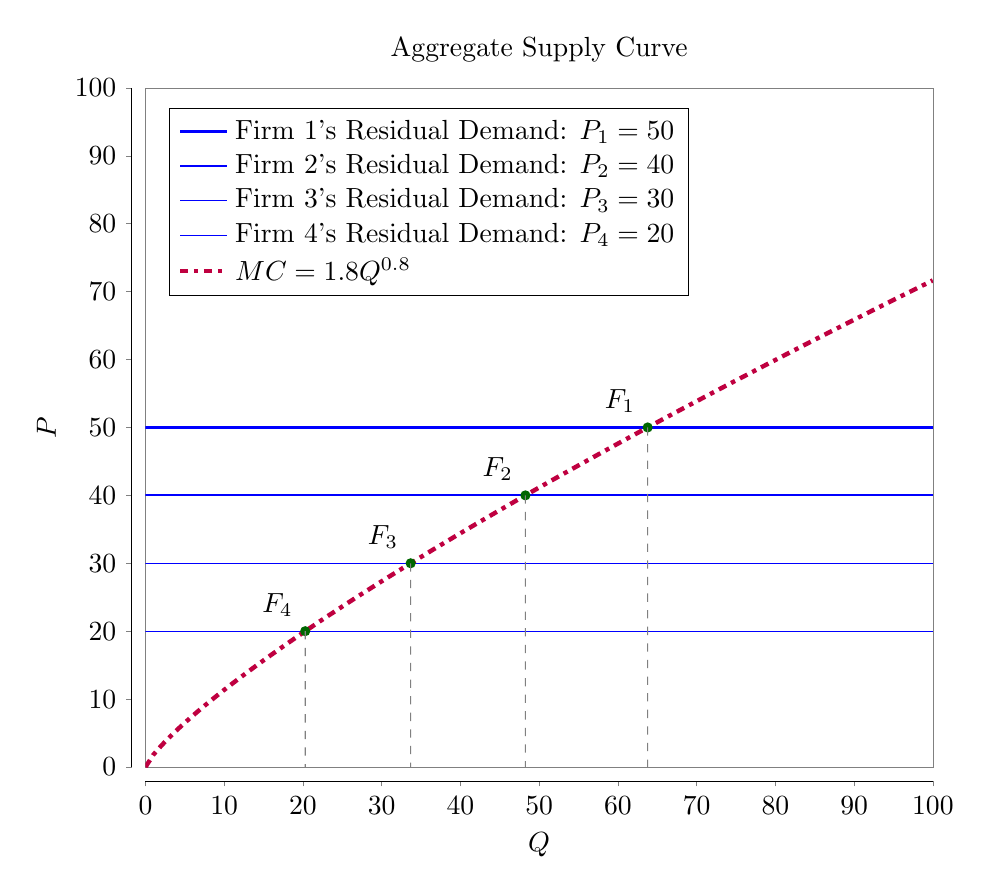
\begin{tikzpicture}

\begin{axis}[
    xmin = 0,
    xmax = 100,
    ymin = 0,
    ymax = 100,
    xlabel = {$Q$},
    ylabel = {$P$},
    sciclean/.style={axis lines=left,
        axis x line shift=0.5em,
        axis y line shift=0.5em,
        axis line style={-,very thin},
        axis background/.style={draw,ultra thin,gray},
        tick align=outside,
        major tick length=2pt},
    xtick distance=10,
    ytick distance=10,
    title = {Aggregate Supply Curve},
    domain = 0:100,
    legend cell align = left,
    legend pos = north west,
    sciclean]

    \addplot[name path = C1, very thick, color = blue, samples = 100] {50};
    \addlegendentry{Firm 1's Residual Demand: $P_{1} = 50$}
    \addplot[name path = C2, thick, color = blue, samples = 100] {40};
    \addlegendentry{Firm 2's Residual Demand: $P_{2} = 40$}
    \addplot[name path = C3, thin, color = blue, samples = 100] {30};
    \addlegendentry{Firm 3's Residual Demand: $P_{3} = 30$}
    \addplot[name path = C4, very thin, color = blue, samples = 100] {20};
    \addlegendentry{Firm 4's Residual Demand: $P_{4} = 20$}

    \addplot[name path = MC, ultra thick, color = purple, dashdotted, samples = 100] {1.8*x^0.8};
    \addlegendentry{$ MC = 1.8 Q^{0.8} $}

    \path[name intersections={of = MC and C1, by=C1MC}];
    \node[fill=black!60!green,circle,inner sep=1.3pt, label={[align=left] 120:$F_{1}$ }] at (C1MC)  {};
    \Getxycoords{C1MC}{\xRC}{\yRC}
    \draw[dashed, gray] (C1MC) -- (\xRC, 0);

    \path[name intersections={of = MC and C2, by=C2MC}];
    \node[fill=black!60!green,circle,inner sep=1.3pt, label={[align=left] 120:$F_{2}$ }] at (C2MC)  {};
    \Getxycoords{C2MC}{\xRC}{\yRC}
    \draw[dashed, gray] (C2MC) -- (\xRC, 0);

    \path[name intersections={of = MC and C3, by=C3MC}];
    \node[fill=black!60!green,circle,inner sep=1.3pt, label={[align=left] 120:$F_{3}$ }] at (C3MC)  {};
    \Getxycoords{C3MC}{\xRC}{\yRC}
    \draw[dashed, gray] (C3MC) -- (\xRC, 0);

    \path[name intersections={of = MC and C4, by=C4MC}];
    \node[fill=black!60!green,circle,inner sep=1.3pt, label={[align=left] 120:$F_{4}$ }] at (C4MC)  {};
    \Getxycoords{C4MC}{\xRC}{\yRC}
    \draw[dashed, gray] (C4MC) -- (\xRC, 0);

    % \path[name path = xRC] (\xRC, 0) -- (\xRC, 100);
    % \path[name intersections={of = D and xRC, by=DxRC}];
    % \node[fill=black!60!green,circle,inner sep=1.3pt, label={[align=left] 60:$D$ }] at (DxRC)  {};
    % \Getxycoords{DxRC}{\DxRC}{\DyRC}
    % \draw[dashed, gray] (\xRC, 0) -- (DxRC) -- (0, \DyRC);


\end{axis}


\end{tikzpicture}

\end{document}
